\documentclass{article}
\usepackage[utf8]{inputenc}
\usepackage[left=1cm,right=0.5cm,bottom=0.5cm,top=0.5cm]{geometry}
\usepackage{setspace}
\usepackage{graphicx}
\usepackage{amsmath}
\usepackage{graphbox}
\usepackage{enumitem}
\setstretch{0.8}
\setlist{nosep}

% 2 sides of paper
\begin{document}
\begin{center}
    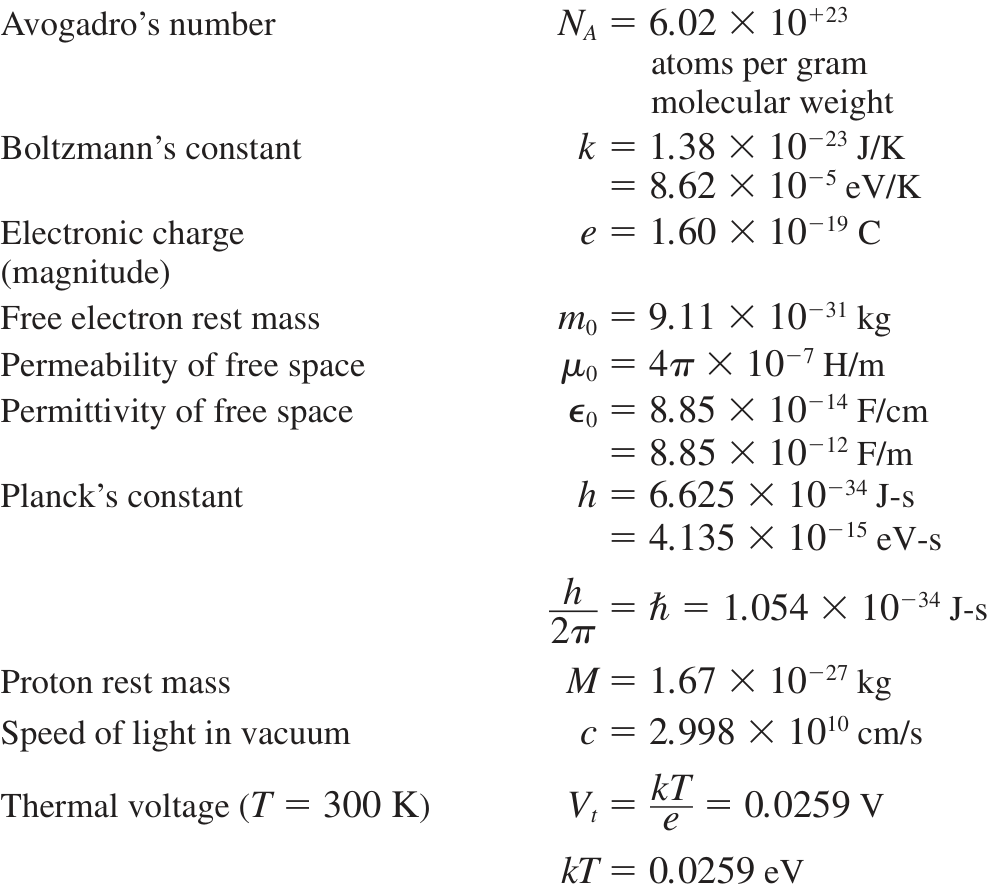
\includegraphics[align=c, height=7cm, width=6cm]{consts.png}
    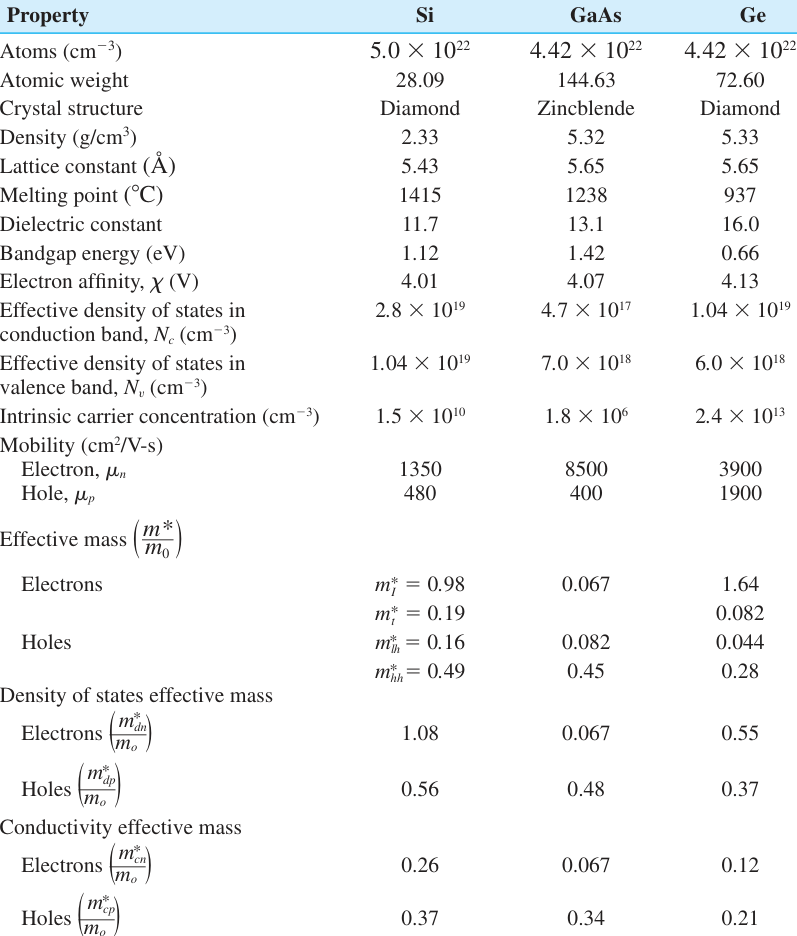
\includegraphics[align=c, height=7cm, width=6cm]{props.png}
    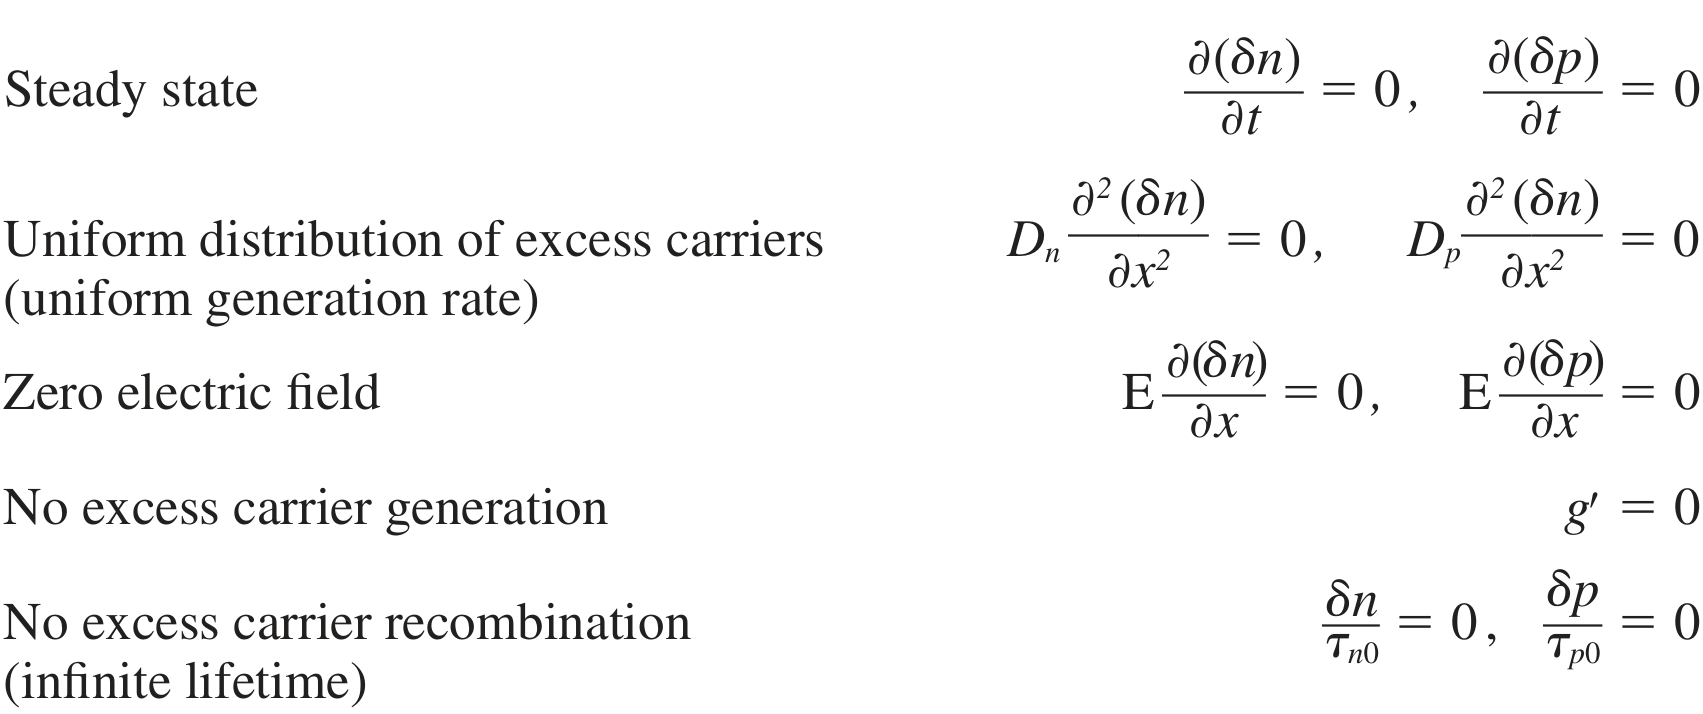
\includegraphics[align=c, height=7cm, width=7cm]{continuity.png}
\end{center}
\textbf{Basics of solids}
\begin{itemize}
    \item $E_c$ is the min energy of the conduction band, $E_v$ is the max energy of the valence band, $E_g$ is the bandgap ($E_c - E_v$)
    \item Density of states
    \begin{itemize}
        \item Conduction band: $g_c(E) = \frac{4 \pi (2m_n^*)^{3/2}}{h^3} \sqrt{E - E_c}$, Valence band: $g_v(E) = \frac{4 \pi (2m_p^*)^{3/2}}{h^3} \sqrt{E_v - E}$
    \end{itemize}
    \item Fermi-Dirac probability
    \begin{itemize}
        \item Probable distribution function: $f_F(E) = \frac{1}{1 + exp\left(\frac{E - E_F}{kT}\right)}$
        \item $f_F(E_F) = \frac{1}{2}$, and $E_F$ is known as the Fermi energy. Kind of the "center" of the distribution
        \item Boltzmann approx (when $E - E_F >> kT$): $f_F(E) \approx exp\left[\frac{-(E - E_F)}{kT}\right]$
    \end{itemize}
\end{itemize}
\textbf{Dopants}
\begin{itemize}
    \item Intrinsic means no dopants at all, extrinsic means doped. Complete ionization is assumed for all dopants.
    \item When $n_0 > p_0$, semiconductor is N-type (majority donors), and when $p_0 > n_0$, semiconductor is P-type (majority acceptors)
    \item Thermal equilibrium carrier concentrations
    \begin{itemize}
        \item Electron concentration (unit is $cm^{-3}$): $n_0 = N_c \cdot exp\left[\frac{-(E_c - E_F)}{kT}\right] = n_i \cdot exp\left[\frac{E_F - E_{Fi}}{kT}\right]$, $n_0 \propto N_c = 2\left(\frac{2 \pi m_n^* kT}{h^2}\right)^{3/2}$
        \item Hole concentration (unit is $cm^{-3}$): $p_0 = N_v \cdot exp\left[\frac{-(E_F - E_v)}{kT}\right] = p_i \cdot exp\left[\frac{-(E_F - E_{Fi})}{kT}\right]$, $p_0 \propto N_v = 2\left(\frac{2 \pi m_p^* kT}{h^2}\right)^{3/2}$
        \item $N_c$ and $N_v$ are the "effective density of states", and are \textbf{very temperature dependent} with $N = N_{T0} \cdot \frac{T}{T_0}^{3/2}$.
        \item For an intrinsic semiconductor, $n_i = p_i$, and $n_i^2 = N_c N_v exp\left[\frac{-E_g}{kT}\right] = N_c N_v exp\left[\frac{-(E_c - E_v)}{kT}\right]$
        \item For intrinsic AND extrinsic semiconductors, $n_0 \cdot p_0 = n_i^2$
    \end{itemize}
    \item Compensated semiconductors
    \begin{itemize}
        \item $n_0 = \frac{N_d - N_a}{2} + \sqrt{\left(\frac{N_d - N_a}{2}\right)^2 + n_i^2}$, $p_0 = \frac{N_a - N_d}{2} + \sqrt{\left(\frac{N_a - N_d}{2}\right)^2 + n_i^2}$
    \end{itemize}
    \item Fermi energy modelling
    \begin{itemize}
        \item For an intrinsic semiconductor, $E_{Fi} - E_{midgap} = \frac{3}{4} kT \ln \left(\frac{m_p^*}{m_n^*}\right)$
        \item We can use the $n_0$ functions: $E_c - E_F = kT \ln \left(\frac{N_c}{n_0}\right)$, $E_F - E_{Fi} = kT \ln \left(\frac{n_0}{n_i}\right)$ (n-type)
        \item We can use the $p_0$ functions: $E_F - E_v = kT \ln \left(\frac{N_v}{p_0}\right)$, $E_{Fi} - E_F = kT \ln \left(\frac{p_0}{n_i}\right)$ (p-type)
    \end{itemize}
\end{itemize}
\textbf{Carrier drift}
\begin{itemize}
    \item $J_{drf} = e(\mu_n n + \mu_p p)E = \sigma \cdot E$, $\rho = \frac{1}{\sigma} = \frac{1}{e(\mu_n n + \mu_p p)}$. N-type and P-type $n >> p$, $p >> n$ applies for simplification
    \item $J_{diff} = J_{n|diff} + J_{p|diff}$, $J_{n|diff} = e D_n \nabla{n} = e D_n \frac{dn}{dx}$ (in 2D), $J_{p|diff} = -e D_p \nabla{p} = -e D_p \frac{dp}{dx}$ (in 2D)
    \item $J = J_{drf} + J_{diff}$, $\frac{D_n}{\mu_n} = \frac{D_p}{\mu_p} = \frac{kT}{e}$, $\mu$ unit is $\frac{cm^2}{V \cdot s}$, $J$ unit is $\frac{A}{cm^2}$, $D$ unit is $\frac{cm^2}{s}$
    \item Flux is the true direction of electrons and holes. Current is opposite of flux for electrons, same for holes. Use flux for intuition
\end{itemize}
\textbf{Continuity equation}
\begin{itemize}
    \item Diffusion length: $L_p = \sqrt{D_p \tau_p}$, $L_n = \sqrt{D_n \tau_n}$
    \item Low injection means low number of excess carriers vs. equilibrium carriers
    \item P-type under low injection: $D_n \frac{\partial^2(\delta n)}{\partial x^2} + \delta n \mu_n \frac{\partial E}{\partial x} + \mu_n E \frac{\partial (\delta n)}{\partial x} + g' - \frac{\delta n}{\tau_{n0}} = \frac{\partial (\delta n)}{\partial t}$
    \item N-type under low injection: $D_p \frac{\partial^2(\delta p)}{\partial x^2} - \delta p \mu_p \frac{\partial E}{\partial x} - \mu_p E \frac{\partial (\delta p)}{\partial x} + g' - \frac{\delta p}{\tau_{p0}} = \frac{\partial (\delta p)}{\partial t}$
    \item $g'$ is generation, $\frac{\delta n}{\tau_{n0}}$ is recombination ($\tau_{n0}$ is the excess carrier lifetime), $D_n \dots$ is diffusion, $\mu_n E \dots$ is drift
    \item Case 1: Steady state, no generation process, no drift ($g' = 0, \frac{\partial}{\partial t} = 0, E = 0$) $\rightarrow \delta n(x) = A \cdot e^{-x/L_N} + B \cdot e^{x/L_N}$
    \item Case 2: No drift and no carrier gradient ($\frac{\partial}{\partial x} = 0, E = 0$) $\rightarrow \delta n(t) = G_L \tau_n \left(1 - e^{-t/\tau_n}\right) + \delta n(0) e^{-t/\tau_n}$
    \item Case 3: Steady state, no generation process, no drift, no recombination ($g' = 0, \frac{\partial}{\partial t} = 0, E = 0, \tau_n \rightarrow \infty$) $\rightarrow \delta n(x) = A + B \cdot x$
    \item Case 4: No additional carrier generation process and uniform E field ($g' = 0, \frac{\partial E}{\partial x} = 0$) $\rightarrow \delta n(x, t) = A \cdot \frac{e^{-t/\tau_n}}{\sqrt{4 \pi D_N t}} \exp\left[- \frac{\left(x - \mu_n E t\right)^2}{4 D_N t}\right]$
\end{itemize}
\textbf{P-N diode}
\begin{itemize}
    \item Built-in voltage (V): $V_{bi} = \frac{kT}{e} \ln \left(\frac{N_a N_d}{n_i^2}\right)$, total voltage across diode (R = reverse, A = forward): $V_{tot} = V_{bi} + V_R = V_{bi} - V_A$
    \item Depletion lengths (cm): $x_n = \left\{\frac{2 \epsilon_s V_{tot}}{e}\left[\frac{N_a}{N_d}\right]\left[\frac{1}{N_a + N_d}\right]\right\}^{\frac{1}{2}}$, $x_p = \left\{\frac{2 \epsilon_s V_{tot}}{e}\left[\frac{N_d}{N_a}\right]\left[\frac{1}{N_a + N_d}\right]\right\}^{\frac{1}{2}}$, $W = \left\{\frac{2 \epsilon_s V_{tot}}{e}\left[\frac{N_a + N_d}{N_a N_d}\right]\right\}^{\frac{1}{2}}$
    \item Electric field $\left(\frac{V}{cm}\right)$: $E_{max} = -\left\{\frac{2e V_{tot}}{\epsilon_s}\left(\frac{N_a N_d}{N_a + N_d}\right)\right\}^{\frac{1}{2}} = -\frac{2 V_{tot}}{W}$
    \item Electric field: $E(x) = \begin{cases}
        \frac{-q N_A}{\epsilon_s}(x + x_p) & -x_p < x < 0 \\
        \frac{-q N_D}{\epsilon_s}(x_n - x) & 0 < x < x_n \\
        0 & else
    \end{cases}$,
    voltage: $V(x) = \begin{cases}
        0 & x < -x_p \\
        \frac{q N_A}{2 \epsilon_s}(x + x_p)^2 & -x_p < x < 0 \\
        V_{bi} - \frac{q N_D}{2 \epsilon_s}(x_n - x)^2 & 0 < x < x_n \\
        V_{bi} & x > x_n
    \end{cases}$
    \item Positive external voltage shrinks total voltage, negative increases. Depletion length also shrinks and increases accordingly.
    \item Current density $(\frac{A}{cm^2})$: $J = q\left(e^{q V_A / kT} - 1\right)\left[\frac{n_i^2 D_N}{N_A L_N} + \frac{n_i^2 D_P}{N_D L_P}\right]$
\end{itemize}
\begin{center}
    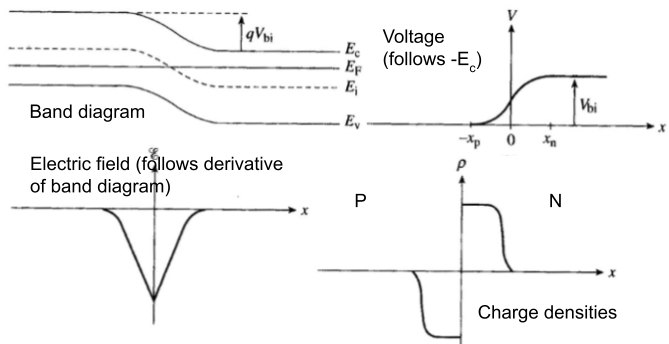
\includegraphics[align=c, height=5.5cm]{pngraphs.png}
    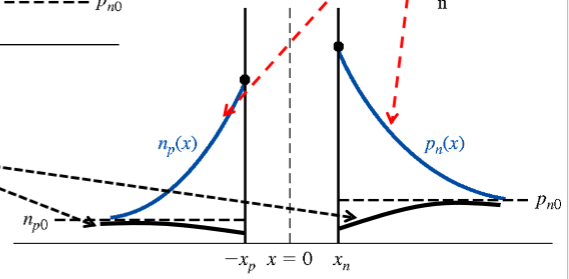
\includegraphics[align=c, height=4.5cm]{pncarriers.png}
\end{center}
\textbf{Bipolar junction transistors (NPN and PNP)}
\begin{itemize}
    \item From left to right: emitter, base, collector. Emitter is more heavily doped, base is more lightly doped, collector is least doped.
    \item Minority current is the determiner of the behavior of the diode. The mode of the diode is entirely based on minority carriers.
    \item Emitter injection efficiency ($\gamma_{npn} = \frac{J_{nE}}{J_{nE} + J_{pE}}$) - Ratio of minority to majority current in emitter. Since minority current changes behavior, want ratio close to 1 so emitter is "efficient" in switching modes.
    \item Base transport factor ($\alpha_{Tnpn} = \frac{J_{nC}}{J_{nE}}$) - Ratio of minority current through collector to emitter. Want close to 1 (no leakage through base).
    \item Approximations for gain factors (ignoring exponential values)
    \begin{itemize}
        \item $\gamma = \frac{1}{1 + \frac{D_E N_B L_B}{D_B N_E L_E} \cdot \frac{\sinh(W / L_B)}{\cosh(W / L_B)}}$
        \item $\gamma \approx \frac{1}{1 + \frac{D_E N_B W}{D_B N_E L_E}}$ if narrow base approx is allowed $(W \ll L_E)$. You can assume sinh is approximately a straight line.
        \item $\alpha_T = \frac{1}{\cosh(W / L_B)}$, Common base current gain - $\alpha_{dc} = \gamma \cdot \alpha_T = \frac{I_C}{I_E}$, Common emitter current gain - $\beta_{dc} = \frac{I_C}{I_B} = \frac{\alpha_{dc}}{1 - \alpha_{dc}}$
        \item $\alpha_T \approx \frac{1}{1 + \frac{1}{2} \cdot \left(\frac{W}{L_B}\right)^2}$ if narrow base approx is allowed, by Taylor series
        \item KCL of the BJT at forward bias: $I_E = I_B + I_C$
    \end{itemize}
\end{itemize}
\begin{center}
    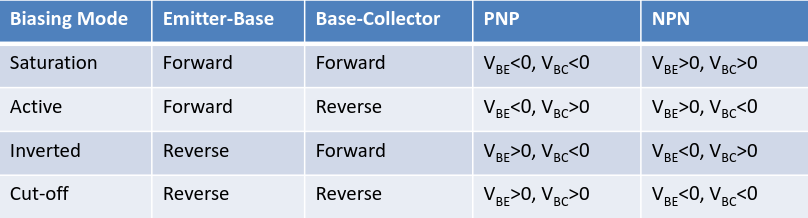
\includegraphics[align=c, height=2.5cm]{bjtvolts.png}
    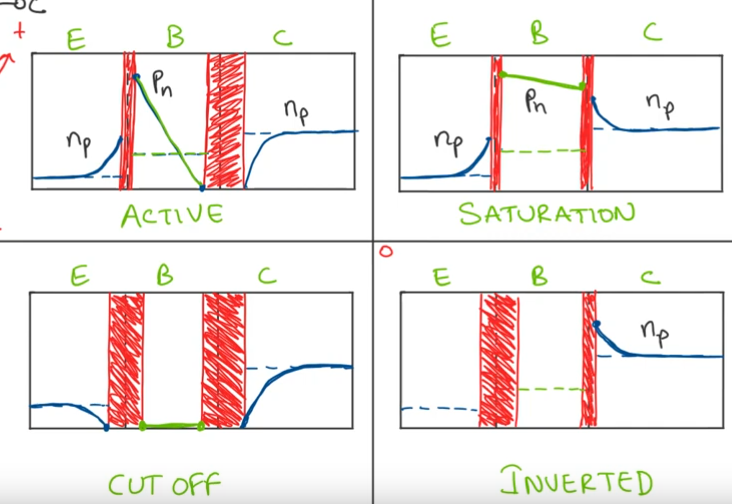
\includegraphics[align=c, height=5.5cm]{pnpcarriers.png}
    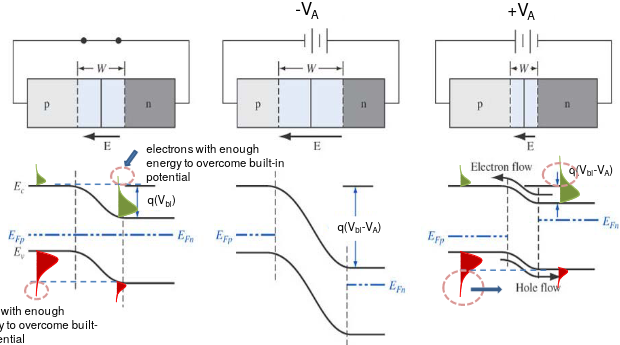
\includegraphics[align=c, height=4.5cm]{pnbias.png}
    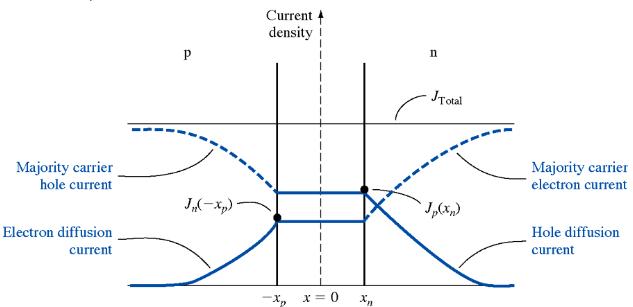
\includegraphics[align=c, height=4.5cm]{pncurrent.png}
    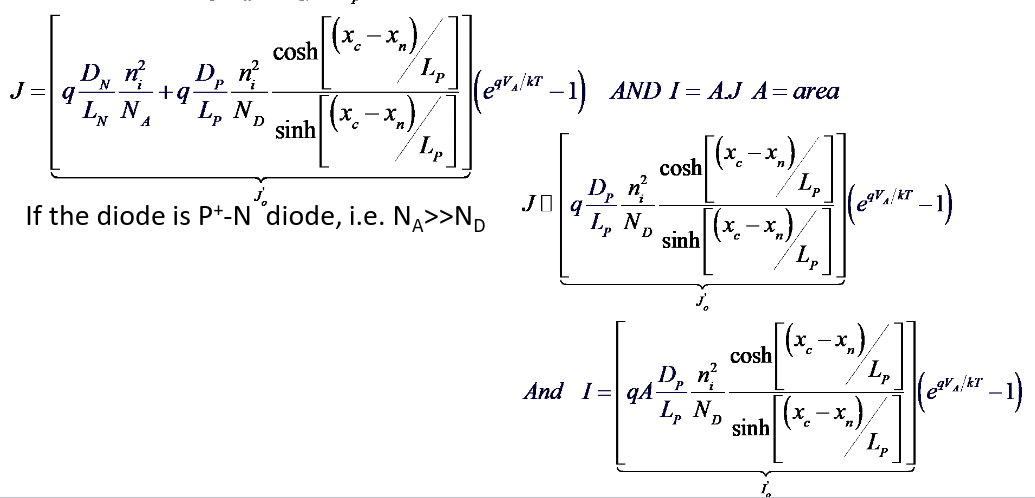
\includegraphics[align=c, height=4.5cm]{narrowcurrent.png}
    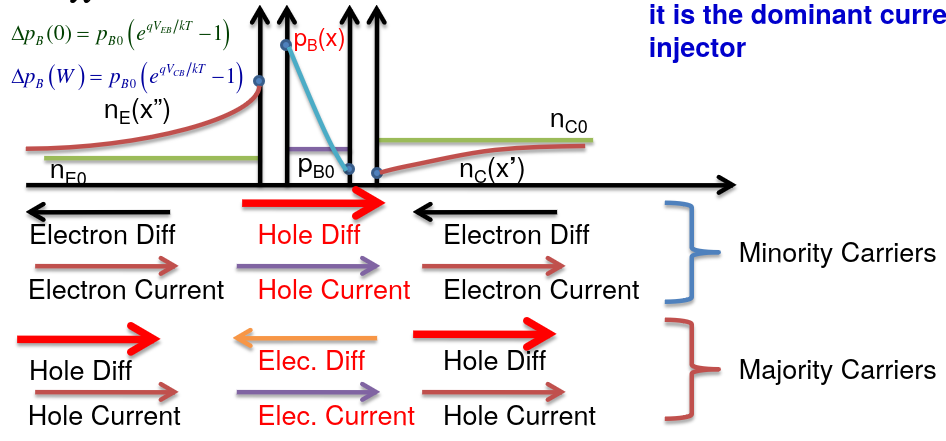
\includegraphics[align=c, height=4.5cm]{pnpfwdcarriers.png}
    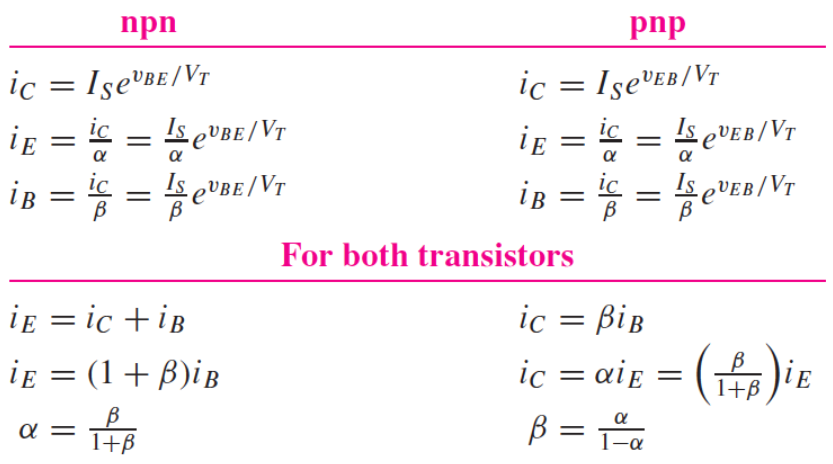
\includegraphics[align=c, height=4.5cm]{bjtcurrents.png}
    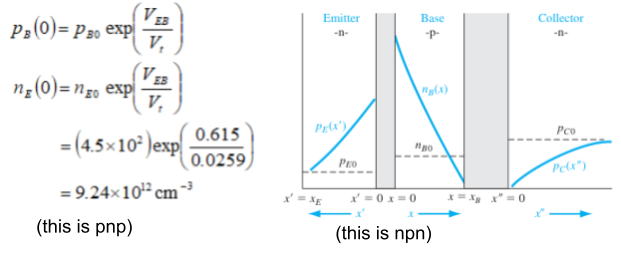
\includegraphics[align=c, height=4.5cm]{bjtcurrenteqs.png}
    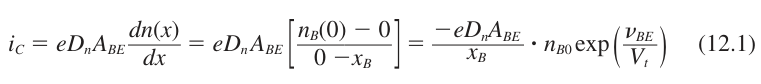
\includegraphics[align=c, height=1cm]{bjtic.png}
    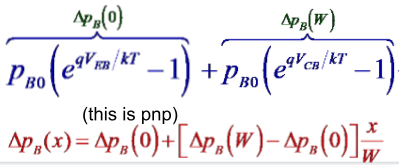
\includegraphics[align=c, height=2cm]{bjtbaseapprox.png}
\end{center}
\textbf{MOS capacitors}
\begin{itemize}
    \item $\phi_b$ is the charge difference between the metal and the vacuum level (where an electron is \textit{detached} from its atom)
    \item $\phi_s$ is the charge difference between the semiconductor's fermi energy and the vacuum level
    \item $\phi_F$ is the charge difference between the intrinsic fermi and fermi levels of the semiconductor side
    \item $\chi$ is the electron affinity and is the voltage difference between the semiconductor's conduction band and the vacuum level
    \item We assume that the MOS is at flat band with no external voltage for convenience ($\phi_b = \phi_s$)
    \item 3 modes: accumulation, depletion, inversion
    \begin{itemize}
        \item Accumulation is when the voltage injects excess carriers of the same charge as the semiconductor
        \item Depletion is when the voltage injects excess carriers of the opposite charge, creating a depletion region
        \item Inversion is past depletion. Now the semiconductor looks like it's doped the opposite direction that it is at equilibrium.
        \item For example, N-type at inversion looks like P-type and P-type at inversion looks like N-type
        \item The boundary between depletion and inversion is $V_G = V_T$ (the gate voltage is equal to the threshold).
    \end{itemize}
    \item Potential difference threshold (external voltage where \textit{no} charge is on the capacitor): $\phi_s = 2 \cdot \phi_F$
    \item Depletion layer width: $W = \sqrt{\frac{2 K_s \epsilon_0}{q N_A} \cdot \phi_s}$, depletion space charge density: $Q'_{SD}(max) = e \cdot N_A \cdot W$ for p-type, $Q'_{SD}(max) = e \cdot N_D \cdot W$ for n-type
    \item Surface potential: $\phi_s = \frac{kT}{q} \cdot \ln\left(\frac{N_A}{n_i}\right)$ for p-type, $\phi_s = \frac{kT}{q} \cdot \ln\left(\frac{N_D}{n_i}\right)$ for n-type
\end{itemize}
\begin{center}
    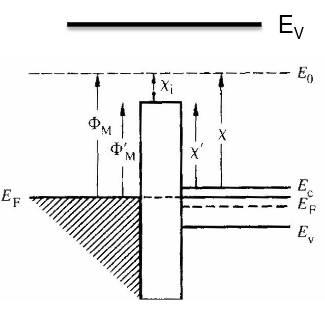
\includegraphics[align=c, width=4.5cm]{mosflat.png}
    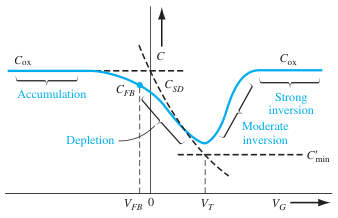
\includegraphics[align=c, width=4.5cm]{moscv.png}
    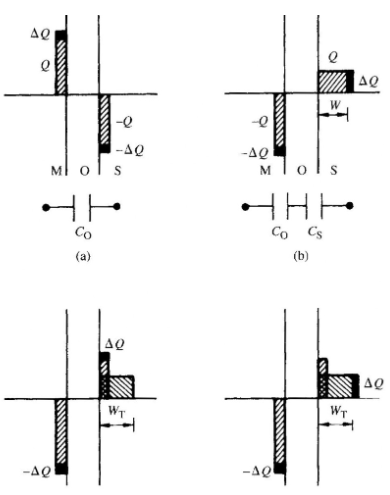
\includegraphics[align=c, width=4.5cm]{moscap.png}
\end{center}
\textbf{MOSFETs}
\begin{itemize}
    \item All of these are in terms of NMOS (n-channel). PMOS uses subscripts of P.
    \item Drain-source saturation voltage: $V_{DS}(sat) = V_{GS} - V_T$
    \item Drain current vs. drain-source voltage: $I_D = \begin{cases}
        \frac{k_n'}{2} \frac{W}{L} \cdot \left[2(V_{GS} - V_T) V_{DS} - V_{DS}^2\right] & V_{DS} < V_{DS}(sat), V_{GS} \geq V_T \\
        \frac{k_n'}{2} \frac{W}{L} \cdot \left[V_{GS} - V_T\right]^2 & V_{DS} \geq V_{DS}(sat), V_{GS} \geq V_T \\
    \end{cases}$
    \item Process conduction parameter (units of $\frac{A}{V^2}$): $k_n' = \mu_n \cdot C_{ox}$, Oxide capacitance (constant, unit of C): $C_{ox} = \frac{\epsilon_{ox}}{t_{ox}}$
\end{itemize}
\begin{center}
    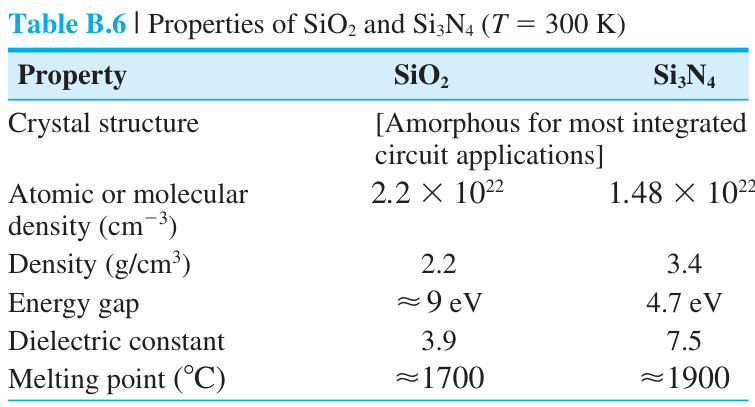
\includegraphics[align=c, height=4.5cm]{oxides.png}
    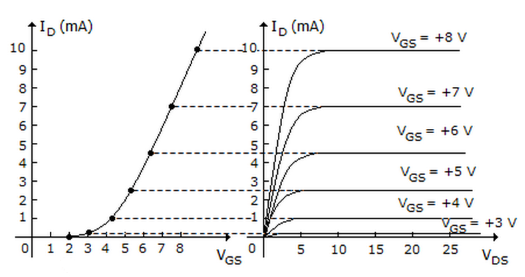
\includegraphics[align=c, height=4.5cm]{mosfetcurves.png}
\end{center}
\end{document}
